\documentclass[11pt,a4paper]{article}

\textwidth=150mm
\textheight=230mm
\topmargin=0pt
\headheight=0pt
\oddsidemargin=3mm
\evensidemargin=0mm
\headsep=0pt
\parindent=0pt
\renewcommand{\baselinestretch}{1.15}
\setlength{\parskip}{0.3\baselineskip plus 1pt minus 1pt}
\renewcommand{\floatpagefraction}{.8}

\usepackage{times}
\usepackage{url}
\usepackage{tikz}
\usepackage{listings}
\usepackage{graphicx}

\lstset{
    language=Python,
    basicstyle=\ttfamily,
    commentstyle=\sffamily\small,
    numberstyle=\scriptsize,
    identifierstyle=\ttfamily,
    showstringspaces=true,
    xleftmargin=3mm,
    escapechar=?,
    sensitive=true,
    breaklines=true,
    firstnumber=last,
    numbers=left,
    numbersep=3mm,
    frame=lines,
    framexleftmargin=5mm,
    columns=fullflexible,
}

% progln{title} - env for program with title and line numbers
\lstnewenvironment{progln}[1]
  {\lstset{firstnumber=auto,name=#1,title={\normalsize\sf #1}}}
  {}
% proglnn{title} - env for continuation of program
\lstnewenvironment{proglnn}[1]
  {\lstset{name=#1}}{}
% prog  - environment for program fragment
\lstnewenvironment{prog}
  {\lstset{numbers=none,}}{}
% Inline program text delimited by ^
\lstMakeShortInline[identifierstyle=\ttfamily\small]^
% \li   - line number
\newcommand*{\li}[1]{{\footnotesize\textsf{\ddag #1}}}

% Font for buttons and menus
\newcommand*{\bu}[1]{\textsf{\small #1}}

\begin{document}

\thispagestyle{empty}

\begin{sffamily}
\begin{center}
\begin{LARGE}
\textbf{A Tutorial on Programming\\\bigskip
the Thymio Robot in Python}
\end{LARGE}

\bigskip

Version 0.1

\begin{Large}
\bigskip\bigskip\bigskip\bigskip
\textbf{Moti Ben-Ari}
\end{Large}

\bigskip\bigskip

\textbf{\url{http://www.weizmann.ac.il/sci-tea/benari/}}

\end{center}
\end{sffamily}

\vfill

\begin{center}
\copyright{}\  2022 by Moti Ben-Ari. 
\end{center}
\begin{small}
This work is licensed under the Creative Commons Attribution-ShareAlike 3.0 Unported License. To view a copy of this license, visit \url{http://creativecommons.org/licenses/by-sa/3.0/} or send a letter to Creative Commons, 444 Castro Street, Suite 900, Mountain View, California, 94041, USA.
\end{small}

\newpage
\setcounter{tocdepth}{2}
\tableofcontents

\thispagestyle{empty}
\newpage
\setcounter{page}{1}

%%%%%%%%%%%%%%%%%%%%%%%%%%%%%%%%%%%%%%%%%%%%%%%%%%%%%%%%%%

\section{Introduction}\label{s.introduction}

The Thymio II robot can be programmed in graphical languages for novices (VPL, VPL3, Blockly, Scratch) and in textual languages for those with experience in programming (Aseba, Python). This document is a tutorial on programming the Thymio II robot using Python. The subset of the Python language supported by the Thymio is sufficient to implement advanced algorithms such as those in \cite{elements}. Complete references on programming the Thymio are \cite{native,thymio,tdm}.

The document assumes the following knowledge and skills:
\begin{itemize}
\item Familiarity with the Thymio that you can obtain by exploring the pre-programmed behaviors and by constructing programs in one of the graphical languages such as VPL.

\item The ability to write elementary programs in Python.
\end{itemize}

Python programs can be written using the Thonny integrated development environment (IDE).\footnote{The Jupyter IDE can also be used to develop Python programs for the Thymio.} Thonny is recommended because it is similar to other IDEs that you may have used.

The Python programs are processed as shown in Figure~\ref{f.architecture}.
\begin{figure}[hb]
\begin{center}
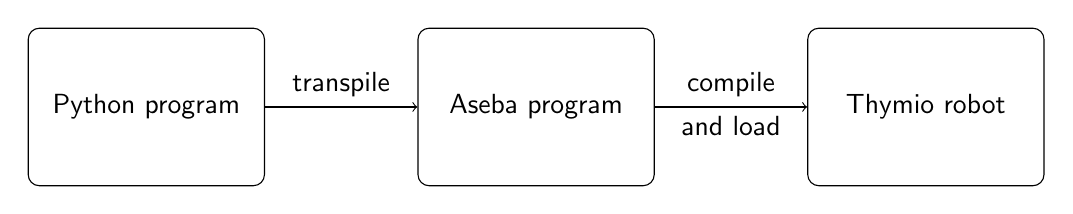
\begin{tikzpicture}[scale=.9]
\node (p) at (0,0)
  [draw,rectangle,rounded corners,
   minimum width=3cm,minimum height=2cm]
   {\sf Python program};
\node (a) at (5.5,0)
  [draw,rectangle,rounded corners,
   minimum width=3cm,minimum height=2cm]
   {\sf Aseba program};
\node (t) at (11,0)
  [draw,rectangle,rounded corners,
   minimum width=3cm,minimum height=2cm]
   {\sf Thymio robot};
\draw[->] (p.east) -- node[above] {\sf transpile} (a.west);
\draw[->] (a.east) -- node[above] {\sf compile}
                      node[below] {\sf and load} (t.west);
\end{tikzpicture}
\end{center}
\caption{The architecture of the Thymio Python environment}\label{f.architecture}
\end{figure}


A \emph{transpiler} translates the Python program into a program in the Aseba language which was the original programming language for the Thymio. Fortunately, this step is transparent and you don't have to learn Aseba.

The Thymio Suite compiles and loads programs into the Thymio. You will already have used Thymio Suite to run programs written in VPL. For Python you need to run Thymio Suite initially but no further interaction is needed.

Section~\ref{s.installation} explains how to install the software  for programming the Thymio and Section~\ref{s.running} explains how to run a program. Section~\ref{s.example} is an extended example that demonstrates Python programming for the Thymio. Section~\ref{s.subset} lists the constructs of Python that are supported by the Thymio and Section~\ref{s.interface} describes the events, variables and functions used to interface with the Thymio. Section~\ref{s.variables} shows how to display the values of Thymio variables.

\textbf{Acknowledgment} I am deeply indebted to Yves Piguet for his untiring help.

\newpage

%%%%%%%%%%%%%%%%%%%%%%%%%%%%%%%%%%%%%%%%%%%%%%%%%%%%%%%%%%

\section{Installation}\label{s.installation}

Download and install the Thymio Suite:
\begin{center}
\url{https://www.thymio.org/download-thymio-suite-redirect/}
\end{center}
If you have written graphical programs for the Thymio the software will already be installed.

\begin{description}
\item[Windows] Run the \texttt{exe} installation file.
\item[MacOS] Open the \texttt{dmg} file, then drag and drop the \bu{ThymioSuite.app} icon onto the Applications icon in the same window:
\begin{center}
\includegraphics*[width=.4\textwidth]{mac-installation.png}
\end{center}
\item[Linux] Follow the instructions at \url{https://www.thymio.org/linux-installation/}.
\end{description}

Download and install the Thonny environtment:\footnote{Thonny bundles a Python interpreter in its installation. Should you wish to use a different interpreter (at least version 3.6), after installing Thonny select the menu item  \bu{\footnotesize Run/Select interpreter} and then \bu{\footnotesize Alternative Python 3 interpreter or virtual environment}.}
\begin{center}
\url{https://thonny.org/}
\end{center}
When you run it for the first time select the menu item \bu{Tools/Manage plug-ins}. In the search bar write \verb+tdmclient-ty+ and select \bu{Search on PyPI}. In the search results select \verb+tdmclient-ty+ which will install the plugin. Select \bu{Close} when the installation is finished.

%%%%%%%%%%%%%%%%%%%%%%%%%%%%%%%%%%%%%%%%%%%%%%%%%%%%%%%%%%

\section{Running a Python program}\label{s.running}

\begin{enumerate}
\item Attach the Thymio to the computer with a USB cable or a wireless dongle. Turn on the Thymio by touching the center button for several seconds.
\item Run Thymio Suite which will connect the Thymio software with the computer. You can select the icon \bu{Aseba Studio} to verify that the Thymio is recognized although this is not necessary.
\item Run Thonny. By default three panes are shown: (i) the central pane with tabs for each open source file, (ii) the \bu{Shell} pane below where printed output will be displayed, (iii) the \bu{Assistant} pane on the right displays hints on compilation errors and warnings.
\item The Thonny interface is standard with commands for opening and closing files, editing, searching, replacing, and so on. You can run and debug a regular Python program using the commands in the \bu{Run} menu.
\item The menu \bu{Thymio} contains four commands for running Python programs on the Thymio:
\begin{enumerate}
\item \bu{Run}: Transpile and run a Python program. Interact with the Thymio as you would if it were programmed in VPL. Output from ^print^ statements will appear in the \bu{Shell}.
\item \bu{Transpile program}: Transpile a Python program. If transpiler does not find any errors, the Aseba program that results will be  displayed in the \bu{Shell}. You do not need to examine it.
\item \bu{Stop}: Stop the running of your program in the Thymio. This may not stop the motors so be sure to include a way of stopping them like the button event handler \li{14-30} in the example below.

\item \bu{Unlock}: See \cite{tdm}.
\end{enumerate}

\end{enumerate}

%%%%%%%%%%%%%%%%%%%%%%%%%%%%%%%%%%%%%%%%%%%%%%%%%%%%%%%%%%

\section{An extended example}\label{s.example}

We implement a \emph{Braitenberg vehicle} displaying the \emph{dogged} behavior \cite[Chapter~3]{elements}. Several versions of the program, each adding some feature, will be given. The programs are split into sections and each is explained separately.

Notation: \li{n} refers to line \textsf{n} of the program.

\subsection*{The initial program}

\begin{progln}{Dogged behavior}
"""
  Braitenberg vehicle: dogged behavior

  When the robot detects an object in front it moves backwards
  When the robot detects an object in back it moves forwards

  The robot is turned on and off using the center button
    When turned on, initially the robot moves forwards
    When turned off, the robot stops
"""

# State: False = off, True = on
state = False
\end{progln}

The program starts with comments describing its behavior. A global variable ^state^ is ``declared'' at \li{13}. In Python variables are not declared but come into being when they are assigned a value.

\begin{proglnn}{Dogged behavior}
# Event handler for the center button
@onevent
def button_center():
    # Global declarations
    global state
    global motor_left_target, motor_right_target

    # The variable button_center is False if the button is released
    if not button_center:
        if state:
            state = False
            motor_left_target = 0
            motor_right_target = 0
        else:  # not state
            state = True
            motor_left_target = 200
            motor_right_target = 200
\end{proglnn}

Most programming for the Thymio is done within \emph{event handlers} which are run when the associated event occurs. An event handler is syntactically a function \emph{without} parameters, prefixed with the \emph{decorator} ^@onevent^ \li{15}.

The center button starts and stops the program. The event handler ^button_center()^ \li{16} is called whenever the button is touched (^button_center^ receives the value ^False^) or released (^button_center^ receives the value ^True^). The event handler uses three predefined variables: ^motor_left_target^ and ^motor_right_target^ which are used to set the power of the motors, and ^button_center^ \li{22} which contains data associated with the event. 

When the button is released ^state^ is toggled off to on or on to off, and the motors powers are set either to move forwards \li{29-30} or to stop \li{25-26}.

Since both ^state^ and the motor powers are global variables that are modified, they must be declared ^global^. The variable ^button_center^ is only read so it need not be declared ^global^.

\newpage

\begin{proglnn}{Dogged behavior}
# Event handler for proximity sensors
@onevent
def prox():
    # Global declarations
    global motor_left_target, motor_right_target

    # If state is off don't do anything
    if not state: return

    # If front central sensor detects an object
    #   set motors to move backwards
    if prox_horizontal[2] > 2000:
        motor_left_target = -200
        motor_right_target = -200
    # If both back sensors detect an object
    #   set motors to move forwards
    elif prox_horizontal[5] > 2000 and \
         prox_horizontal[6] > 2000:
        motor_left_target = 200
        motor_right_target = 200
\end{proglnn}

The behavior is implemented in an event handler that reads the front center horizontal proximity sensor and the two rear horizontal proximity sensors. Nothing is done if the Thymio is off \li{38}.

The values of the sensors are stored in ^prox_horizontal^ which holds seven values: values detected by the five front sensors and the values detected by the two rear sensors (Figure~\ref{f.robot}). If an object is detected in front of the Thymio \li{42}, the motors are reversed from forwards to backwards; if the object is behind the Thymio \li{47-48}, the motors are reversed from backwards to forwards.

Recall that to continue a line in Python \li{47} you must use the backslash character. Alternatively, parentheses can be used:
\begin{prog}
    elif (prox_horizontal[5] > 2000 and
            prox_horizontal[6] > 2000):
\end{prog}

\begin{figure}[t]
\begin{center}
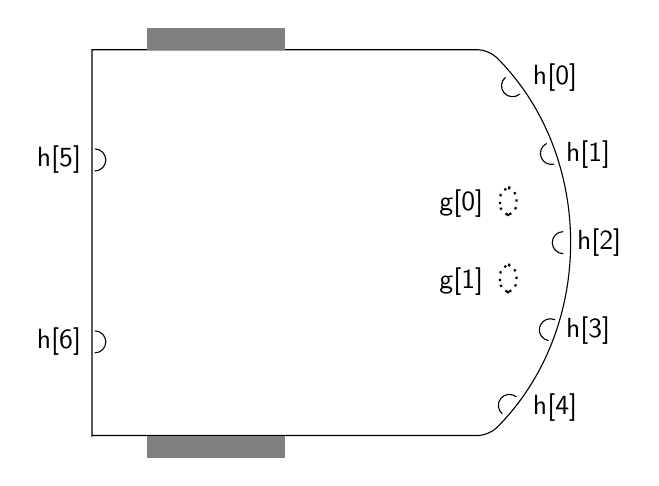
\begin{tikzpicture}[scale=.7]
% Robot body
\draw (-2.2cm,-3.5cm) to [rounded corners] (5cm,-3.5cm) to%
[rounded corners, bend right=45] (5cm,3.5cm) to (-2.2cm,3.5cm) to cycle;
% Wheels
\fill[gray] (-1.2cm,-3.5cm) rectangle +(2.5cm, -.4cm);
\fill[gray] (-1.2cm,3.5cm) rectangle +(2.5cm, .4cm);
% Front horizontal sensors
\draw (5.3, 3)
  arc[start angle=130, end angle=310, radius=.2cm];
\draw (6.05, 1.8)
  arc[start angle=115, end angle=285, radius=.2cm];
\draw (6.35, .2)
  arc[start angle=90, end angle=270, radius=.2cm];
\draw (6.2, -1.4)
  arc[start angle=65, end angle=260, radius=.2cm];
\draw (5.5, -2.8)
  arc[start angle=50, end angle=230, radius=.2cm];
% Rear horizontal sensors
\draw (-2.15, 1.7)
  arc[start angle=90, end angle=-90, radius=.2cm];
\draw (-2.15, -1.6)
  arc[start angle=90, end angle=-90, radius=.2cm];
% Ground sensors
\draw[thick,dotted,rounded corners] (5.2, .5)
  rectangle +(.3,.5);
\draw[thick,dotted,rounded corners] (5.2, -.9) 
  rectangle +(.3,.5);
% Labels
\node at (6.2,3) {\sf h[0]};
\node at (6.8,1.6) {\sf h[1]};
\node at (7,0) {\sf h[2]};
\node at (6.8,-1.6) {\sf h[3]};
\node at (6.2,-3) {\sf h[4]};
\node at (-2.8,1.5) {\sf h[5]};
\node at (-2.8,-1.8) {\sf h[6]};
\node at (4.5,.7) {\sf g[0]};
\node at (4.5,-.7) {\sf g[1]};
\end{tikzpicture}
\end{center}
\caption{The sensors of the Thymio robot: \textsf{h=horizontal, g=ground}}\label{f.robot}
\end{figure}

\subsection*{Displaying the state in the top LEDs}

Let us modify the program so that the top LEDs will display the state of the program, not just the value of ^state^ but also if the Thymio is moving forwards or backwards. The color displayed by the top LEDs can be set by calling a function with three arguments giving the color as a combination of (red, green, blue) each in the range 0 to 32. Add the following function calls after the numbered line in the above program:

\newpage

\begin{prog}
nf_leds_top(32,32,32)  ?$\;$? # White, line 24
nf_leds_top(0,0,0)     ?$\quad\quad\,$? # Off,   line 28
nf_leds_top(0,32,0)    ?$\quad\;\;$? # Green, line 42
nf_leds_top(0,0,32)    ?$\quad\;\;$? # Blue,  line 48
\end{prog}

\subsection*{Defining a function}

Instead of writing calls to the Thymio function inline, let us place a single call in a function so that we can change the display operation for all uses in one place:
\begin{prog}
# Function for setting the top LEDs
def top(r,g,b):
    nf_leds_top(r,g,b)
\end{prog}
Replace all calls to ^nf_leds_top(r,g,b)^ by ^top(r,g,b)^.

\subsection*{The circle LEDs}

The 8 circle LEDs that surround the buttons are extremely useful when programming the Thymio, because they can display small numbers 0 to 8 directly without encoding in colors.\footnote{Larger numbers can be display in binary encoding.} Function ^nf_leds_circle^ takes 8 parameters, one for each LED in the circle, giving the intensity of that LED from 0 to 32. Since it is hard to distinguish levels of intensity, it is recommended to turn each LED either off (0) or on (32). The following function will display the four motion states in the first four circle LEDs:
\newpage

\begin{prog}
def circle(motion):
    if motion == 0: nf_leds_circle(0,0,0,0,0,0,0,0)
    if motion == 1: nf_leds_circle(32,0,0,0,0,0,0,0)
    if motion == 2: nf_leds_circle(32,32,0,0,0,0,0,0)
    if motion == 3: nf_leds_circle(32,32,32,0,0,0,0,0)
\end{prog}
The function call is ^circle(m)^ where the argument ^m^ is a value between 0 and 3.

\subsection*{A clever function}

Instead of a sequence of ^if^-statements we can compute whether a LED is turned off or on:
\begin{prog}
def circle(motion):
    nf_leds_circle(
        32*(motion % 4 > 0),
        32*(motion % 4 > 1),
        32*(motion % 4 > 2),
        0,0,0,0,0)
\end{prog}
The call to ^nf_leds_circle^ will turn on the first three LEDs:
\begin{prog}
0 0 0
32 0 0
32 32 0
32 32 32
\end{prog}


%%%%%%%%%%%%%%%%%%%%%%%%%%%%%%%%%%%%%%%%%%%%%%%%%%%%%%%%%%

\section{The Python subset supported by the Thymio}\label{s.subset}

The only data type is ^int^ which are $16$-bit integers in the range $(-32768,32767)$.

Lists of integers can be accessed as complete lists or as individual elements:
\begin{prog}
a = [0,1,2,3]  # a is a list of integers
print(a[2])    ?$\quad\:$?# Select an individual element
b = a          ?\hspace{53pt}?# Assign an array
print(len(b))  # len is supported
b = a[0:2]  ?$\quad\;\;\;$?# Slices are not supported
print(b)   ?$\quad\quad\;\;$? # Expressions with lists not are supported
\end{prog}

The ^str^ type and the string library functions are not supported but a string can be printed:
\begin{prog}
speed = ...
print('Speed = ', speed)
\end{prog}
Strings can be used for documentation \li{1-10}.

The ^bool^ type is supported.

The undefined value ^None^ is not supported.

Both local and global variables are supported, but since the event handlers do not have parameters you will use global variables more often than in a regular Python program. Do not forget to declare a variable as ^global^ if you change its value inside a function including event handlers.

Arithmetic operations (^a+b^), assignment operations (^a=b^, ^a+=b^), comparisons (^a!=b^), bitwise operations (^a|b^), and the functions ^abs^ and ^len^ are supported. The division operation is integer division with truncation (^a//b^). 

All the control statements are supported with the following exceptions:
\begin{itemize}
\item ^for^ loops are limited to a range of integers (possibly with two or three arguments). The following program prints 10 and then 20:
\begin{prog}
a = [0,10,20,30]
for i in range(1,3):
    print(a[i])
\end{prog}
\item The ^break^ and ^continue^ statements are not supported.
\end{itemize}
Functions can be defined and called but only with positional arguments that are scalars.

%%%%%%%%%%%%%%%%%%%%%%%%%%%%%%%%%%%%%%%%%%%%%%%%%%%%%%%%%%

\section{Interfacing with the Thymio}\label{s.interface}

There are a large number of events, variables and functions that are predefined and used to interface with the Thymio robot. This section will explain some frequently used ones. You can look up the rest of them in the Thymio documentation \cite{thymio}.

\subsection{Events}

Table~\ref{t.events} shows events that cause an event handler to be called.\footnote{Hz, an abbreviation for \emph{hertz}, is the number of times per second that the events occurs. For $20$ Hz the event occurs every $1/20=0.05$ seconds or $50$ milliseconds.}

\begin{table}[t]
\renewcommand{\arraystretch}{.85}
\begin{center}
\begin{tabular}{|l|l|}
\hline
Event& When occurs\\\hline
^button_center^& pressed or released\\
^button_forward^&\\
^button_backward^&\\
^button_left^&\\
^button_right^&\\
\hline
^prox^&periodically 20 Hz\\
^acc^&periodically 16 Hz\\
\hline
^timer0^&timer 0 expired\\
^timer1^&timer 1 expired\\
^sound_finished^&sound duration expired\\
\hline
\end{tabular}
\end{center}
\caption{Events}\label{t.events}
\end{table}

\subsection{Variables}

Table~\ref{t.variables} shows predefined variables. They are all global.
\begin{table}[hbt]
\renewcommand{\arraystretch}{.85}
\begin{center}
\begin{tabular}{|l|l|l|}
\hline
Variable& Meaning & Values\\\hline
^button_center^&State of the center button&True = touched\\
^button_forward^&State of the forward button&False = released\\
^button_backward^&State of the backward button&\\
^button_left^&State of the left button&\\
^button_right^&State of the right button&\\
\hline
^prox_horizontal^&Light reflected&$\sim(0,4000)$\\
&to the horizontal sensors&\\
&An array with 7 elements&\\
\hline
^prox_^&Light reflected&$\sim(0,400)$\\
\hspace{15pt}^ground_delta^&to the ground sensors&\\
&An array with 2 elements&\\
\hline
^acc^&Acceleration along an axis&$(-32,32)$\\
^acc[0]^&x-axis (roll)& left is $+$, right is $-$\\
^acc[1]^&y-axis (pitch)& back is $+$, front is $-$\\
^acc[2]^&z-axis& down is $+$, up is $-$\\
\hline
^motor_^&Set power of left motor&$(-500,500)$\\
\hspace{15pt}^left_target^&&\\
^motor_^&Set power of left motor&\\
\hspace{15pt}^right_target^&&\\
\hline
^timer_period[0]^&Set period of timer 0&Milliseconds\\
^timer_period[1]^&Set period of timer 1&\\
\hline
\end{tabular}
\end{center}
\caption{Predefined variables}\label{t.variables}
\end{table}

\subsection{Predefined functions}

Table~\ref{t.functions} shows predefined functions. They are prefixed with the string ^nf_^, an abbreviation for \emph{native function}. The LED functions take arguments whose values are between 0 and 32. The top and bottom LEDs display colors. The arguments for primary and secondary colors are:
\begin{center}
\begin{tabular}{lccc}
Color & Red & Green & Blue\\\hline
White & 32 & 32 &32\\
Red & 32 & 0 & 0\\
Green & 0 & 32 &0\\
Blue & 0 &0 &32\\
Yellow & 32 & 32 & 0\\ 
Magenta & 32 & 0 & 32\\
Cyan & 0 & 32& 32\\
(off) & 0 & 0 & 0
\end{tabular}
\end{center}
Other colors can be specified using values other than 0 and 32.

The LEDs can also be set by assigning lists to variables:
\begin{center}
\begin{tabular}{|ll|}
\hline
^leds_top^ &^= [r, g, b]^\\
^leds_circle^& ^= [i0, i1, i2, i3, i4, i5, i6, i7]^\\
\hline
\end{tabular}
\end{center}

\begin{table}[hbt]
\renewcommand{\arraystretch}{.85}
\begin{center}
\begin{tabular}{|l|l|}
\hline
Function& Action\\\hline
^nf_leds_top(r,g,b)^&Set top LEDs to $(r,g,b)$ color\\
^nf_leds_bottom_left(r,g,b)^&Set bottom left LEDs to  $(r,g,b)$ color\\
^nf_leds_bottom_right(r,g,b)^&Set bottom right LEDs to $(r,g,b)$ color\\
\hline
^nf_leds_circle(^& Set circle LEDs $n=0..7$\\
\hspace{20pt}^i0,i1,i2,i3,i4,i5,i6,i7)^& \hspace{10pt} to intensity $i_n$\\
\hline
^nf_sound_freq(f,d)^&Plays sound of $f$ hertz\\
&\hspace{15pt}for $d/60$ seconds\\
&\hspace{15pt}$d=0$ continuous sound\\
&\hspace{15pt}$d=-1$ stop sound\\
\hline
\end{tabular}
\end{center}
\caption{Predefined functions}\label{t.functions}
\end{table}

\subsection{Math functions}

Table~\ref{t.math} lists predefined mathematical functions. Many of them have a version prefixed with ^nf_^ which can be used on lists (arrays) of integers \cite{native}. Arguments are 16-bit signed integers as are the returned values.

\begin{table}[htb]
\renewcommand{\arraystretch}{.85}
\begin{center}
\begin{tabular}{|l|l|}
\hline
Function& Returned value\\\hline
^math_rand()^& Random\\
^math_muldiv(a,b,c)^& $(a*b)//c$ \\
^math_sqrt(a)^&$\sqrt{a}$\\
\hline
^math_sin(a)^&$\sin a$\\
^math_cos(a)^&$\cos a$\\
\hline
\end{tabular}
\end{center}
\caption{Math functions}\label{t.math}
\end{table}

\subsection{Calculating with integers}

Suppose that you have set the variable ^motor^ to a power level and wish to reduce it by $25\%$. The computation in \li{2} results in an error because floating-point numbers are not supported. The computation in \li{3} is not correct because it first performs the integer division resulting in $0$ and therefore ^motor1^ will also receive the value $0$. The correct way of performing the calculation is shown in \li{4}. By first performing the multiplication, we obtain $1350$, which, when divided by $4$, results in $337$, very close to the exact value $337.5$.

\begin{progln}{16-bit integer computations}
motor = 450
motor1 = motor * 0.75
motor1 = motor1 * (3//4)
motor1 = (motor*3)//4
motor1 = math_muldiv(motor,3,4)
\end{progln}

Be careful not to overflow $16$-bit computations. $12000\cdot 3=36000$ is too large to fit in a $16$-bit integer. The value stored represents the negative integer $-22760$.  The math function ^math_muldiv^ \li{5} performs the intermediate computation ^a*b^ using 32-bit integers without overflow.

The arguments of the trigonometric functions are 16-bit integers representing radians $(-\pi,\pi)$:
\[
\renewcommand*{\arraystretch}{1.3}
\begin{array}{lccccccc}
\textsf{Radians}&-\pi&-\pi/2&-\pi/4&0&\pi/4&\pi/2&\pi\\\hline
\textsf{Integer}&-32768&-16384&-8192&0&8192&16384&32767\\
\end{array}
\]
The results of the trigonometric functions are 16-bit integers representing $(-1.0,1.0)$:
\[
\renewcommand*{\arraystretch}{1.3}
\begin{array}{lccccccc}
\textsf{Radians}&-\pi&-\pi/2&-\pi/4&0&\pi/4&\pi/2&\pi\\\hline
\textsf{sin(rad)} & 0 & -1.0 & -\sqrt{2}/{2} & 3 & \sqrt{2}/{2} & 1.0& 0\\
\textsf{sin(int)}&0&-32767&-23171&0&23171&32767&0\\\hline
\textsf{cos(rad)} & -1.0 & 0 & \sqrt{2}/{2} & 1.0 & \sqrt{2}/{2} & 0& -1.0\\
\textsf{cos(int)}&-32767&0&23171&32767&23171&0&-32767\\
\end{array}
\]

An important advantage of programming the Thymio in Python is that you can develop and test computations offline using the ``regular'' Python interpreter. For example, suppose that you want to specify a scaling factor for the computation of distance from motor power and time. The following Python statements can be run without a robot (use the commands from the Thonny menu \bu{Run}):

\newpage

\begin{prog}
motor  ?$\;\;$? = 300     # motor power
time   ?$\quad\:$? = 100    # time between samples in milliseconds
samples = 6      ?$\;\;$? # number of samples
scale  ?$\;\;$?  = 600    # set to a value that gives distance in cm

print(motor * time)
print((motor * time) // scale)
print(((motor * time) // scale) * samples)
\end{prog}
The computations are performed one-by-one to check for overflow.
%%%%%%%%%%%%%%%%%%%%%%%%%%%%%%%%%%%%%%%%%%%%%%%%%%%%%%%%%%

\section{Displaying the variables}\label{s.variables}

It is often helpful to display the values of Thymio's variables explicitly. For example, you may want to observe the precise values returned by the sensors in order to calibrate an algorithm. All the variables can be displayed by running the program \texttt{tdmclient.tools.gui} \cite{tdm}. Normally you will just want to examine a few variables such as the sensors. This can be done by running a small program which prints the values of selected variables:
\begin{progln}{Displaying variables}
timer_period[1] = 500

def print_horizontal():
    print('prox_horizontal',
          prox_horizontal[0], prox_horizontal[1],
          prox_horizontal[2], prox_horizontal[3],
          prox_horizontal[4],
          prox_horizontal[5], prox_horizontal[6])
def print_ground():
    print('prox_ground_delta',
          prox_ground_delta[0], prox_ground_delta[1])
def print_accelerometers():
    print('acc: roll = ', acc[0],
          'pitch = ', acc[1],
          'vertical = ', acc[2])

@onevent
def timer1():
    print_horizontal()
    print_ground()
    # print_accelerometers()
\end{progln}

Set one of the timers to a duration (in \li{1} it is set to 500ms which is 0.5s) so that it is easy to observe the values as they are printed. Define functions \li{3-15} to print the variables you have selected. Finally, a timer event handler \li{17-21} calls these functions at the specified interval. If you only need to display some of these variables you can comment-out the others as in \li{21}.

You can add these statements to your own programs assuming that you use only one timer.

%%%%%%%%%%%%%%%%%%%%%%%%%%%%%%%%%%%%%%%%%%%%%%%%%%%%%%%%%%

\bibliographystyle{plain}
\begin{small}
\bibliography{python-tutorial}
\end{small}
\end{document}
